\documentclass[a4paper,11pt,makeidx]{report} % Font size

\usepackage{makeidx}
\usepackage{color}
\usepackage{listings}
\usepackage{graphicx}
\usepackage{hyperref}
\usepackage[nohyphen]{underscore}

\hypersetup{colorlinks=true}
%%% AH Macros
\long\def\comment#1{}
\def\pipkw{\tt\bf\color{blue}}%
\def\pipterm#1{\index{#1}{\pipkw #1}}%
\def\PIPID{\pipterm{PIPID}}%
\def\NULL{\tt NULL}%

\lstloadlanguages{C,csh}

\lstset{basicstyle=\small\tt, numberbychapter=true, showstringspaces=false,
  emph={pip_get_pipid, pip_get_ntasks,
    pip_init, pip_fin,
    pip_spawn, pip_wait, pip_wait_any,
    pip_task_spawn, pip_spawn_program_t,
    pip_spawn_from_func, pip_spawn_from_main, 
    pip_named_export, pip_named_import, pip_exit, 
    pip_barrier_init, pip_barrier_wait, pip_barrier_fin,
    pip_barrier_t, pip_gettime,
    PIP_PIPID_ROOT, PIP_PIPID_ANY, PIP_PIPID_MYSELF, 
    PIP_CPUCORE_ASIS, PIP_MODE_PTHREAD, PIP_MODE_PROCESS,
    pip-exec, pipcc, pipfc, pip-mode, printpipmode}, 
  emphstyle={\pipkw}, texcl=true, escapeinside={<(}{)>}}


\lstdefinestyle{program}{numbers=none, numberstyle=\tiny, numbersep=5pt, frame=tb, language=C}
\lstdefinestyle{example}{numbers=none, numberstyle=\tiny, numbersep=5pt, language=, frame=tRBl}
\lstdefinestyle{define}{frame=single, language=csh}

\title{Great Experiences with PiP} % Book title
\author{Atsushi Hori} % Author

%--------------------------------------------------------------------------------
\makeindex

\begin{document}
\maketitle

\newpage % Make sure the following content is on a new page

%----------------------------------------------------------------------------------------
%	TABLE OF CONTENTS
%----------------------------------------------------------------------------------------

\tableofcontents % Prints the table of contents
\lstlistoflistings
\listoffigures
\listoftables

\chapter{PiP Basics}


\section{Introduction}

blablabla


\section{PiP Tasks}

This section will explain how PiP tasks are created simply and how
they operate differently from processes (made using \term{MPI}) and
threads (created using \term{OpenMP}).

\subsection{\PIPKW{pipcc} and \PIPKW{pip-exec} Commands}
\label{sec:pipcc-exec}

The first example is  the well-known C program ``hello world'' listed
below; 

\lstinputlisting[style=program, caption={Hello World
    ({\tt hello.c})},label=prg:hello] {tasks/examples/hello.c}

As you can see, this program is a perfect match for a standard C
program. If the \pipcmd{pipcc} command was used to compile the
program, it can be run as a standard C program or as a PiP task by
using the \pipcmd{pip-exec} command.

\lstinputlisting[style=example, 
  caption={Hello World - Compile and Execute}, label=out:hello]
                {tasks/examples/hello.out}

A true C compiler can be called with the proper options, such as {\tt
  -I}, {\tt -L}, and others, using the \pipcmd{pipcc} command, which
is written as a shell script. You will see the options available when
the \pipcmd{pipcc} script calls the backend C/C++ compiler if the {\tt
  —silent} option is omitted. 

In this case, \pipcmd{pip-exec} is being used to run an executable
file as PiP tasks rather than a standard Linux process.  
The hello program does not operate differently in the process and PiP
task in this case. In the following section, we'll talk about this
issue.

\subsection{Comparing MPI, OpenMP and PiP}

We slightly alter the ``hello world'' software as follows to clarify the
distinction between the Linux process and PiP task;

\lstinputlisting[style=program,
  caption={Hello World having a static variable ({\tt hello-var.c})},
  label=prg:hello-var] {tasks/examples/hello-var.c}

Now, the address of the static variable {\tt x} in the ``Hello World''
program is printed out along with the message "Hello World." The
number of PiP jobs to be created and run concurrently can be set using
the \pipcmd{pip-exec} command option. In the execution example that
follows, the number three (3) is supplied. The same {\tt a.out}
execution using MPI's output is also included. It should be noted that
the ``Hello World'' program runs in parallel with \pipcmd{pip-exec}
and \mpi{mpiexec}.  

\lstinputlisting[style=example, 
  caption={Hello World with a static variable - Compile and Execute},
  label=out:hello-var] {tasks/examples/hello-var.out}

The variable {\tt x} is found at the address {\tt 0x5555556010301}
according to the first execution of a.out. With MPI execution, this
circumstance is same\footnote{For simplicity, we disabled ASLR
  (Address Space Layout Randomization) in this example.}. The variable
{\tt x} is however executed at various places for each 
PiP activity. This is due to \term{MPI} jobs not sharing the same address
space as PiP tasks.

Readers who are curious in the distinction between
PiP and \term{OpenMP} may observe that threads also share the same address
space. The ``Hello World'' program with a static variable is shown in
the example below written in \term{OpenMP}.

\lstinputlisting[style=program,
  caption={Hello World in OpenMP ({\tt hello-var-omp.c})},
  label=prg:hello-var-omp] {tasks/examples/hello-var-omp.c}

The output of program~\ref{prg:hello-var-omp}'s execution is displayed
below. The addresses of variable {\tt x} in this case are the same for
\term{MPI} and \term{OpenMP} executions. The variable's addresses with
PiP execution, however, are different pairings.

\lstinputlisting[style=example, 
  caption={Hello World in OpenMP, PiP and MPI - Compile and Execute},
  label=out:hello-var-omp] {tasks/examples/hello-var-omp.out}

These variations are explained in
Figure~\ref{fig:tasks:hello-var-omp}. The variable {\tt x} is shared 
by all of the \term{OpenMP} threads, and they all use the same address
space. Each \term{MPI} process in an MPI environment has its own address
space, and two (2) threads can execute in each address space while
sharing a variable in an MPI process. However, each PiP task has its
own variables, thus threads 0 and 1 only share variables within the
same PiP task; they do not share variables inside any other PiP
tasks. In PiP, all PiP tasks share the same address space.

\begin{figure}[ht]
\centering
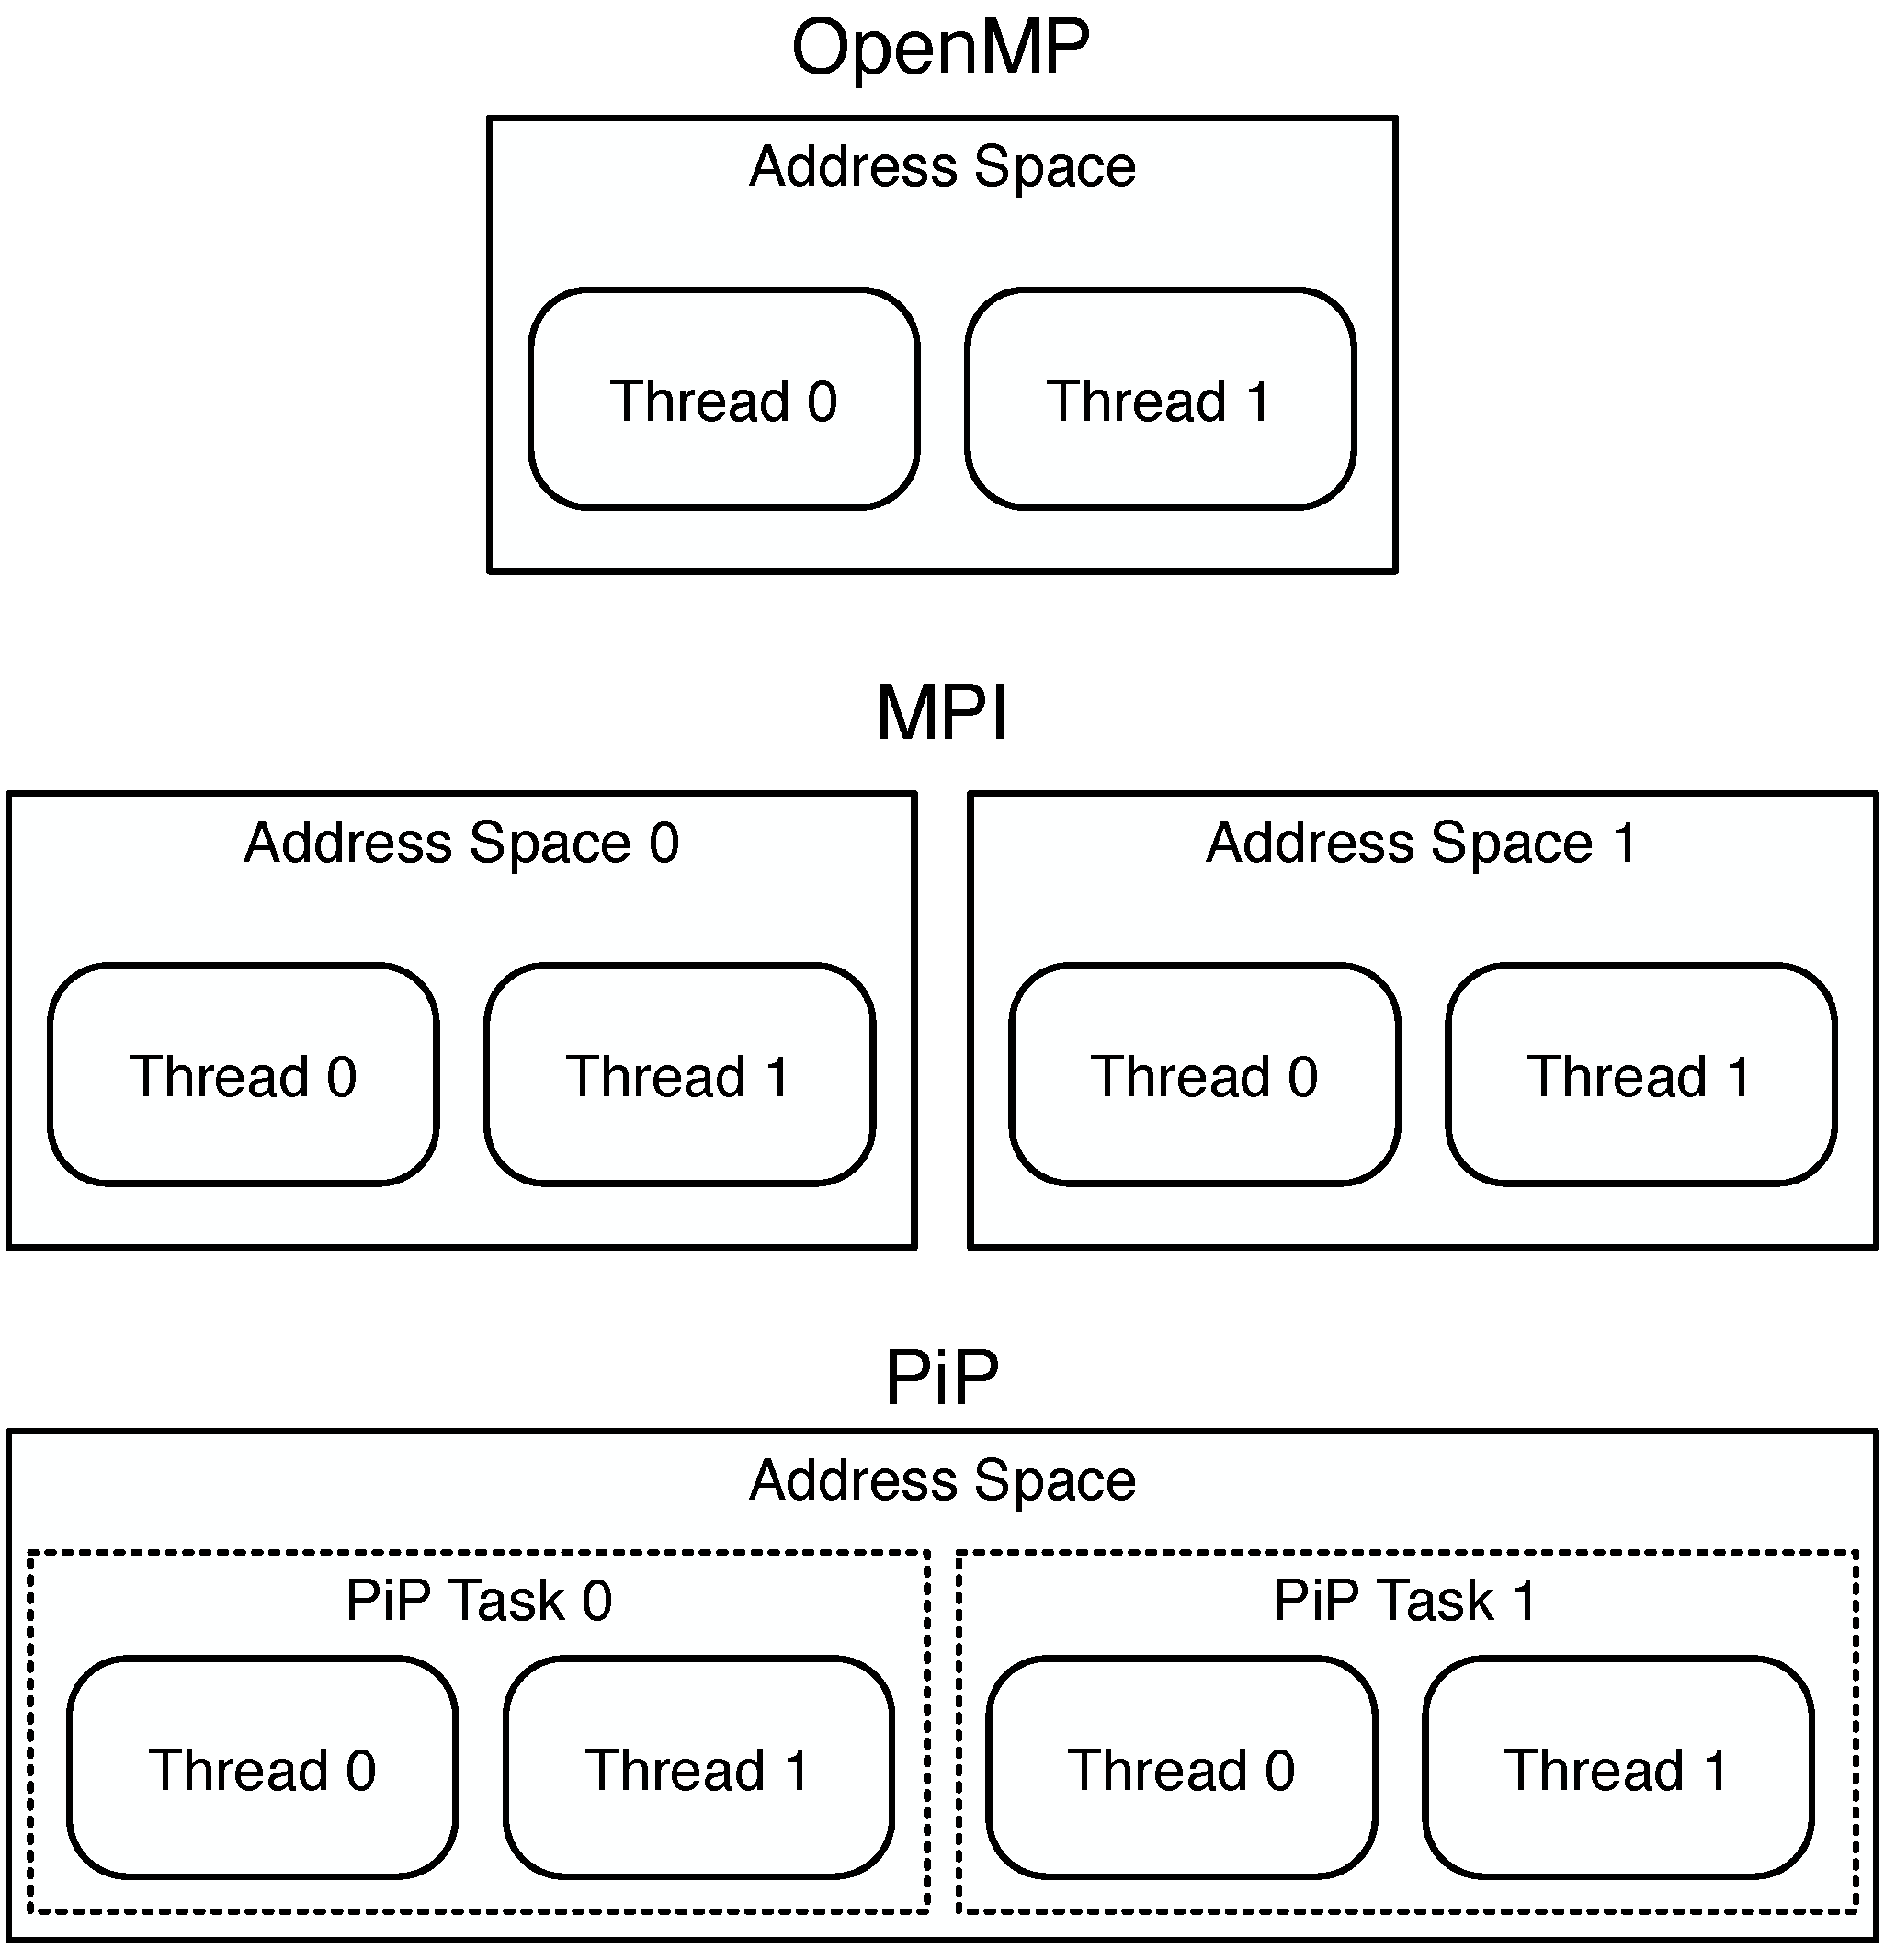
\includegraphics[width=0.7\columnwidth]{tasks/Figs/AddressSpace-OpenMP-MPI-PiP.pdf}
\caption{Differences of OpenMP, MPI and PiP}
\label{fig:tasks:hello-var-omp}
\end{figure}

Static variables are associated to an address space in the traditional
process model and thread model. Because of this, each process has its
own static variables, which are shared by all threads using the same
address space. Each PiP task is guaranteed to have its own static
variable set under the PiP execution model, decoupling from the
address space while maintaining address space sharing. {\it variable
  privatization} is what this is.

It is simple to share information among PiP tasks while maintaining
the independence of each PiP task's execution thanks to the nature of
PiP, which includes privatized variables and sharing an address
space. The ``Hello World'' program has so far been proved to be able to
execute as PiP tasks concurrently, although this program is quite
basic and there is no information exchange between PiP tasks. We'll
demonstrate how information can be shared between PiP processes in the
section after this one.

\subsection{Export and Import}

If the address of the information to be exchanged is known, sharing an
address space allows data owned by a PiP task to be accessed. The
address of the shared data can be broadcast by a PiP task, and the
other PiP task(s) can obtain the published address.  

To start, each PiP task has a {\PIPID} that helps it stand out from the
rest. By giving the {\PIPID} of the exporting PiP task, other PiP tasks
that share the same address space can import the exported address.

\lstinputlisting[style=program,
  caption={Export and Import ({\tt export-import})},
  label=prg:export-import] {tasks/examples/export-import.c}

In this program, after adjusting the value of {\tt argv[1]}, a PiP
task with a PIPID of zero (zero) exports the address of the variable
{\tt x} by using \pipfunc{pip_named_export}. By using the
\pipfunc{pip_named_import} function, the 
remaining PiP tasks import the address that PiP task 0 exported. An
outcome of this program's execution is shown below. The other PiP
tasks can view the value that PiP task 0 exported, as demonstrated.

\lstinputlisting[style=example, 
  caption={Execution of Export and Import},
  label=out:export-import] {tasks/examples/export-import.out}

The address with the specified name is published by the
\pipfunc{pip_named_export} function. The
\pipfunc{pip_named_import} function blocking-waits for the specified
PiP job by {\PIPID} to reach the defined address. To avoid a race condition,
it is not permitted to export an address with the same name more than
once for the purpose of updating the address.

The PiP library's functions almost always return an integer value as
an error code. A return code of zero (zero) denotes success. This
error code is identical to those that Linux defines. Due to simplicity
and clarity, the returned code is not tested in the examples presented
thus far and moving forward.  

It is forbidden in \term{MPI} to access the data that is held by other
processes running on the same node\footnote{Strictly speaking, some
  \term{MPI} implementations based on the thread model may allow
  this. Major \term{MPI} implementation, such MPICH, 
Open MPI, and many other \term{MPI} implementations provided by vendors are
based on the process model, and there is no way to access data owned by
the other \term{MPI process}.}. In MPI, communication is the sole 
permitted method. Communication fundamentally entails copying data in
some way (done by software or hardware). Data copying consumes memory,
power, and time.



\section{Spawning PiP Tasks and Waiting Terminations}

The \pipcomm{pip-exec} command spawns PiP tasks. The
process which spawns PiP tasks is called {\bf (PiP) root} process. The
\pipcomm{pip-exec} process is a PiP root process. 
PiP tasks spawned by the root process are mapped and executed in the
address space of the root. In this chapter, how to spawn PiP tasks
will be explained.

\subsection{Spawning PiP tasks}

\subsubsection{Spawning a program as PiP tasks}

Listing~\ref{prg:spawn-root} is an example of a PiP root program. It
spawns $N$ PiP tasks, where $N$ is specified by the first parameter
of the program. The \pipfunc{pip_init()} function must be called to
initialize the PiP library before calling any other PiP functions,
although there some exceptions to this. The \pipfunc{pip_init()} may
look strange because this function behaves differently depending
on if it is called from a PiP root or PiP task. The first argument is
output returning {\PIPID} of the calling task. The second input
arguments is to specify the maximum number of spawning PiP tasks. This
second argument becomes output if this is called by a PiP task,
returning the number specified by the root.
The \pipfunc{pip_fin()} function works as the opposite of
\pipfunc{pip_init()}, finalizing PiP library and freeing allocated 
resources. After calling \pipfunc{pip_fin()}, most PiP library
functions return an error code (\linuxdef{EPERM}).
\comment{The other arguments will be explained in the
  Section~\ref{sec:advanced}.} 

The \pipfunc{pip_spawn()} function is called after then. The first and
second arguments are the same with the Linux's \linuxfunc{execve()}
function; the first is to specify the executable file to be executed
and the second argument is to specify the parameters executing the
program. The third is to specify environment variables. When it is
{\NULL}, then value of the Glibc global variable \linuxvar{environ} is
taken. Th fourth argument is to specify the CPU core number to bind
the spawned PiP task and which CPU core. In this example, the value of
\pipdef{PIP_CPUCORE_ASIS} means that the (CPU) core-bind should be
the same with the one when calling \pipfunc{pip_spawn()}. The fifth
is an input and output argument and you can specify \PIPID\ or
set to \pipdef{PIP_PIPID_ANY} so that PiP library can choose
any. After calling \pipfunc{pip_spawn()}, the argument returns the
actual \PIPID. 

\lstinputlisting[style=program, caption={Spawn ({\tt spawn-root})},
  label=prg:spawn-root] {spawn/examples/spawn-root.c}

Listing~\ref{prg:spawn-task} is very similar to the ``Hello World''
program in the previous section. The major difference here is calling
the \pipfunc{pip_init()} function. Unlike root, this function call is
optional in the PiP task program. By calling this, you can get 
{\PIPID} and the number of maximum PiP tasks which are specified by the
root. Linsting~\ref{out:spawn} shows an example of the execution of
Listing~\ref{prg:spawn-root} and \ref{prg:spawn-task}. 

\lstinputlisting[style=program, caption={Spawn ({\tt spawn-task})},
  label=prg:spawn-task]
                {spawn/examples/spawn-task.c}

\lstinputlisting[style=example, 
  caption={Spawn - Execution}, label=out:spawn]
                {spawn/examples/spawn.out}

\subsubsection{Spawning myself}

A program can be both or either PiP root and PiP
task. Listing~\ref{prg:spawn-myself} shows an example of combining the
programs of Listing~\ref{prg:spawn-root} and \ref{prg:spawn-task}. We
hope you can understand the strange behavior of \pipfunc{pip_init()}
function. The PiP root process also acts like a PiP task. It has a
special PIPID, \pipdef{PIP_PIPID_ROOT}. 
Listing~\ref{out:spawn-myself} shows the example of this
execution. 

\lstinputlisting[style=program, caption={Spawn Myself ({\tt spawn-myself})},
  label=prg:spawn-myself]
                {spawn/examples/spawn-myself.c}

\lstinputlisting[style=example, 
  caption={Spawn Myself - Execution}, label=out:spawn-myself]
                {spawn/examples/spawn-myself.out}

\subsubsection{Starting from other than {\tt main}}\label{sec:spawn-func}

PiP tasks start from the {\tt main()} function in the examples so
far. PiP allows for PiP tasks to start user-defined function other
than {\tt main()}. In this case, use the \pipfunc{pip_task_spawn()}
function instead of calling the \pipfunc{pip_spawn()} function.

\lstinputlisting[style=program, caption={Starting from user-defined
    function ({\tt userfunc})},
  label=prg:userfunc] {spawn/examples/userfunc.c}

Listing~\ref{prg:userfunc} is the program of this example. To decrease
the number of arguments to spawn a PiP task, the
\pipstruct{pip_spawn_program_t} structure is defined. This structure
holds all information for spawning a program, including path to
executable file, function name, and so on. To hide the details of the
structure, \pipfunc{pip_spawn_from_func()} function is also defined
to set these information. The user-defined function must have one
argument ({\tt void*}) and return an integer value which is the same
as the return value from the {\tt main()} function.

\lstinputlisting[style=example, 
  caption={Starting from user-defined function - Execution},
  label=out:userfunc] {spawn/examples/userfunc.out}

The \pipfunc{pip_spawn()} was firstly introduced (from version
1). After then, I noticed users can start PiP tasks other than main,
and the \pipfunc{pip_task_spawn()} function was
introduced (from version 2 or later). The
\pipstruct{pip_spawn_program_t} structure must be set 
by calling the \pipfunc{pip_spawn_from_main()} function when
starting from the {\tt main()} function. Listing~\ref{prg:mainfunc} is
the program rewritten version of Listing~\ref{prg:spawn-myself} by
using the \pipfunc{pip_task_spawn()} and
\pipfunc{pip_spawn_from_main()}.

\lstinputlisting[style=program, caption={Starting from main
    function ({\tt mainfunc})},
  label=prg:mainfunc]
                {spawn/examples/mainfunc.c}

\lstinputlisting[style=example, 
  caption={Starting from main function - Execution},
  label=out:mainfunc] {spawn/examples/mainfunc.out}


\subsection{Waiting for Terminations of PiP tasks}

As readers may have already noticed, the \pipfunc{pip_wait()} is the
function to wait for terminations of the spawned PiP tasks. The
\pipfunc{pip_wait()} function acts like the Linux's \linuxfunc{wait()}
function. In many cases, Linux's \linuxfunc{wait()} function works
with PiP tasks, but there is a certain case it does not. So, it is
recommended for users to use \pipfunc{pip_wait()} function.

The argument of the \pipfunc{pip_wait()} is the pointer to an integer
variable, the same with the Linux's \linuxfunc{wait()} call. The
returned integer can be examined by using the Linux's
\linuxdef{WIFEXITED}, \linuxdef{WIFSIGNALED}, \linuxdef{WEXITSTATUS},
\linuxdef{WIFSIGNALED}, and \linuxdef{WTERMISIG} macros. 

\lstinputlisting[style=program, caption={Waiting for specified PiP task
    terminations ({\tt wait})}, label=prg:wait]
                {spawn/examples/wait.c}

\lstinputlisting[style=example, 
  caption={Waiting for specified PiP task terminations - Execution},
  label=out:wait] {spawn/examples/wait.out}

\pipfunc{pip_wait()} waits for the PiP task termination specified by
        {\PIPID}. 
\pipfunc{pip_wait_any()} function can wait for any PiP tasks and
        {\PIPID} and exit status are returned when terminated (See
        Listing~\ref{prg:waitany} and \ref{out:waitany}).
        \pipfunc{pip_trywait()} and \pipfunc{pip_trywait_any()} are
        the non-blocking versions of \pipfunc{pip_wait()} and
        \pipfunc{pip_wait_any()}, respectively. 

\lstinputlisting[style=program, caption={Waiting for any PiP task
    terminations ({\tt waitany})}, label=prg:waitany]
                {spawn/examples/waitany.c}

\lstinputlisting[style=example, 
  caption={Waiting for any PiP task terminations - Execution},
  label=out:waitany] {spawn/examples/waitany.out}


\subsection{Terminating PiP tasks}

PiP tasks and root can terminate their executions by calling
\pipfunc{pip_exit()} function. This function acts like the Linux's
        \linuxfunc{exit()} function. As described above, it is recommended
        to use \pipfunc{pip_exit()} 
        instead of \linuxfunc{exit()}, because the Linux's \linuxfunc{exit()}
        function works in most cases, however, there is a case it does
        not. Listing~\ref{prg:exit} and \ref{out:exit} show the
        example showing how \pipfunc{pip_exit()} works.

\lstinputlisting[style=program, caption={PiP Task Termination
    function ({\tt exit})}, label=prg:exit] {spawn/examples/exit.c}

\lstinputlisting[style=example, 
  caption={PiP Task Termination - Execution},
  label=out:exit] {spawn/examples/exit.out}


\section{Timing Synchronization among PiP Tasks}

This section will explain about the timing synchronization among PiP
tasks.

\subsection{Barrier Synchronization}

Currently, there is only one synchronization method is supported by
the PiP library, it is barrier synchronization. The API of PiP's
barrier synchronization is borrowed from the one found in the PThread
library. There are three functions in PiP,
\pipterm{pip_barrier_init()}, \pipterm{pip_barrier_wait()}, and
  \pipterm{pip_barrier_fin()}, corresponding to {\tt
    pthread_barreir_init()}, {\tt pthread_barrier_wait()} and {\tt
        pthread_barrier_destroy()}, respectively. 

\lstinputlisting[style=program, caption={Barrier Synchronization
    ({\tt barrier})}, label=prg:barrier] {sync/examples/barrier.c}

In Listing~\ref{prg:barrier}, the \pipterm{pip_init()} function is
given a new non-{\tt NULL} value to the third argument. This is
another form of exporting a pointer from the root to spawnd PiP
tasks. In this example, the address of the \pipterm{pip_barrier_t}
static variable is passed to children so that the children can
synchronize by calling \pipterm{pip_barrier_wait()}.

To clarify the effect of the barrier synchronization, the
synchronization takes place only when the second parameter of the
program execution is not given, and then the return values of
\pipterm{pip_gettime()} are shown by PiP tasks. The
\pipterm{pip_gettime()} returns the current value of {\tt
  gettimeofday()} in double format with the unit of seconds.

The example of running of this program is shown in
Listing~\ref{out:barrier}. In the first run, the barrier
synchronization does not take place and large variance can be seen on
the {\tt gettimeofday()} values. In the second run, where the barrier
synchronization takes place, and smaller variance can be seen.

\lstinputlisting[style=example,
  caption={Barrier Synchronization - Execution},
  label=out:barrier] {sync/examples/barrier.out}

\subsection{Using PThread Synchronization}

Users can utilize the synchronization functions on PiP tasks provided
by the PThread library. This is simply because PiP tasks share the
same address space, just like threads.

\subsection{\tt pthread_barrier}

The same barrier synchronization can also be implemented by using the
{\tt pthread_barrier} functions. 
Listing~\ref{prg:pthread-barrier} is the program simply replacing
{\tt pip_barrier} functions with the {\tt pthread_barrier} functions.

\lstinputlisting[style=program,
  caption={Pthread Barrier ({\tt
      pthread-barrier})},label=prg:pthread-barrier]
                {sync/examples/pthread-barrier.c}

\lstinputlisting[style=example, 
  caption={Pthread Barrier - Execution}, label=out:pthread-barrier]
                {sync/examples/pthread-barrier.out}
                
\subsection{\tt pthread_mutex}

Similarly, {\tt pthread_mutex} also works with PiP. 

\lstinputlisting[style=program,
  caption={Pthread Mutex ({\tt
      pthread-mutex})},label=prg:pthread-mutex]
                {sync/examples/pthread-mutex.c}

\lstinputlisting[style=example, 
  caption={Pthread Mutex - Execution}, label=out:pthread-mutex]
                {sync/examples/pthread-mutex.out}


\section{\pipterm{pipcc} and \pipterm{pipfc}}

\section{\pipterm{pip-exec}}

\section{\pipterm{pip-check}}

\section{\pipterm{pips}}

\section{\pipterm{pip-mode} and \pipterm{printpipmode}}



\comment{
  \input{discuss/discuss}

  \chapter{PiP Advanced}
  
\section{Execution Mode}\label{sec:exec-mode}

PiP library is made to function on Linux. According to
Section~\ref{sec:rationale}, it is very dependent on the
\linuxfunc{dlmopen} and \linuxfunc{clone} functions. Particularly, the
\linuxfunc{clone} function is called with a unique set of 
{\tt CLONE} flags. Many Linux variants exist, and some of them do not
support the specified {\tt CLONE} flag combination (for example,
McKernel\footnote{\url{https://github.com/ihkmckernel/mckernel}}). There
are two ways to execute PiP in such an environment: 
one involves executing \linuxfunc{clone} with a particular flag
combination, and the other involves calling \linuxfunc{pthread_create}
to start a PiP task while 
using the standard {\tt CLONE} flag combination. \pipterm{Process
  mode} refers to the former and \pipterm{pthread mode} to the
latter. Both modes keep the fundamental characteristics of the PiP,
including address space sharing and 
flexible privatization.

\subsection{Differences Between Two Modes}

{\tt CLONE} flag combinations ultimately determine the difference in the
PiP execution mode. The {\tt CLONE} flag values \linuxdef{CLONE_FS},
\linuxdef{CLONE_FILES}, \linuxdef{CLONE_SIGHAND}, and
\linuxdef{CLONE_THREAD} are reset, but \linuxdef{CLONE_VM} and
\linuxdef{CLONE_SYSVSEM} are set, in contrast to the 
pthread mode. 

\begin{table}[ht]
  \centering
  \caption{Differences between two modes}\label{tbl:mode-diff}
  \vspace{3mm}
  \begin{tabular}{c||c|c}
    \hline
    & Process Mode & Pthread Mode \\
    \hline
    \hline
    Address Space Sharing & yes & yes \\
    Variable Privatization & yes & yes \\
    File Descriptors (FDs) & not shared & shared \\
    \hline
  \end{tabular}
\end{table}

The primary distinctions between the two modes are shown in
Table~\ref{tbl:mode-diff}. There are a lot more variations, however
the PiP library offers mode-agnostic functions so that users can
develop PiP programs without worrying about the variations in mode.

\begin{table}[ht]
  \centering
  \caption{Mode-Agnostic Functions}\label{tbl:mode-agnostic}
  \vspace{3mm}
  \small
  \begin{tabular}{c||c|c||l}
    \hline
    Mode-Agnostic & Process Mode & Pthread Mode & \multicolumn{1}{c}{note} \\
    \hline
    \pipfunc{pip_exit()} & {\tt exit()} & {\tt pthread_exit()} &
    termination \\
    \pipfunc{pip_wait()} & {\tt wait()} & {\tt pthread_join()} &
    {\tiny wait termination} \\
    \pipfunc{pip_kill()} & {\tt kill()} & {\tt pthread_kill()} & send
    signal \\
    \pipfunc{pip_sigmask()} & {\tt sigprocmask()} & {\tt
      pthread_sigmask()} & signal mask \\
    \pipfunc{pip_signal_wait()} & sigwait() & sigwait() & wait signal
    \\
    \pipfunc{pip_yield()} & {\tt sched_yield()} & {\tt
      pthread_yield()} & yield \\
%%    \pipterm{pip_abort()} & {\tt abort()} & {\tt abort()} & kill all
%%    tasks \\
    \hline
  \end{tabular}
\end{table}

There are also predicate functions for users to know the current
mode listed in Table~\ref{tbl:mode-predicates}.

\begin{table}[ht]
  \centering
  \caption{Execution Mode Predicates}\label{tbl:mode-predicates}
  \vspace{3mm}
  \begin{tabular}{c|c}
    \hline
    Function name & \multicolumn{1}{c}{note} \\
    \hline
    \pipfunc{pip_is_threaded()} & if pthread mode \\
    \pipfunc{pip_is_shared_fd()} & if FDs are shared \\
    \hline
  \end{tabular}
\end{table}

In the current implementation, \pipfunc{pip_is_threaded} and
\pipfunc{pip_is_shared_fd} have the same meaning. There may be
situations in which those two terms have different meanings, so having
those functions is necessary. 

\subsection{How to Specify Execution Mode}

When calling \pipfunc{pip_init} or setting the \pipenv{PIP_MODE}
environment variable at runtime, the execution mode can be
selected. The function prototype 
for the \pipfunc{pip_init} shown below. Up until this point, the first
three arguments have been discussed.

\begin{lstlisting}[frame=tRBl]
int pip_init( int *pipidp,	[IN/OUT]
              int *ntasksp,     [IN/OUT]
              void **root_expp, [IN/OUT]
              int opts );       [IN]
\end{lstlisting}

The final opts parameter can take one of the following values:
\pipdef{PIP_MODE_PROCESS}, \pipdef{PIP_MODE_THREAD}, or both, or
zero. Zero has the same value as {\tt
  \pipdef{PIP_MODE_PROCESS}|\pipdef{PIP_MODE_PTHREAD}}. The
\pipenv{PIP_MODE} environment can be a string that contains the words
"{\tt process}" or "{\tt pthread}." The value of the \pipenv{PIP_MODE}
environment variable is checked when the opts value is zero or the
value of either oring the two. If no environment is specified, the PiP
library picks a suitable one. The environmental value and the ethical
worth cannot be at odds with one another. 


  \input{task-spawn/task-spawn}

  \appendix
  \chapter{PiP Installation}
  
There are several ways to install PiP listed below;

\begin{itemize}
\item Building from source code
\item \pipcmd{pip-pip} command
\item Using \em{Spack}
\end{itemize}

It was scheduled to use RPM (yum)and Docker, but 
they are not available at the time of this writing.

  \chapter{PiP Internals}
  \input{internals/internals}
  
  \bibliography{ref}
}

\printindex

\end{document}
